%%%%%%%%%%%%%%%%%%%%%%%%%%%%%%%%%%%%%%%%%
% Beamer Presentation
% LaTeX Template
% Version 2.0 (March 8, 2022)
%
% This template originates from:
% https://www.LaTeXTemplates.com
%
% Author:
% Vel (vel@latextemplates.com)
%
% License:
% CC BY-NC-SA 4.0 (https://creativecommons.org/licenses/by-nc-sa/4.0/)
%
%%%%%%%%%%%%%%%%%%%%%%%%%%%%%%%%%%%%%%%%%

%----------------------------------------------------------------------------------------
%	PACKAGES AND OTHER DOCUMENT CONFIGURATIONS
%----------------------------------------------------------------------------------------

\documentclass[
	11pt, % Set the default font size, options include: 8pt, 9pt, 10pt, 11pt, 12pt, 14pt, 17pt, 20pt
	%t, % Uncomment to vertically align all slide content to the top of the slide, rather than the default centered
	%aspectratio=169, % Uncomment to set the aspect ratio to a 16:9 ratio which matches the aspect ratio of 1080p and 4K screens and projectors
]{beamer}

\graphicspath{{Images/}{./}} % Specifies where to look for included images (trailing slash required)

\usepackage{booktabs} % Allows the use of \toprule, \midrule and \bottomrule for better rules in tables
\usepackage{tikz}
\usepackage{bbm}
\usepackage{multirow}
%----------------------------------------------------------------------------------------
%	SELECT LAYOUT THEME
%----------------------------------------------------------------------------------------

\usefonttheme[onlymath]{serif}
% Beamer comes with a number of default layout themes which change the colors and layouts of slides. Below is a list of all themes available, uncomment each in turn to see what they look like.

%\usetheme{default}
%\usetheme{AnnArbor}
%\usetheme{Antibes}
%\usetheme{Bergen}
%\usetheme{Berkeley}
%\usetheme{Berlin}
%\usetheme{Boadilla}
% \usetheme{CambridgeUS}
%\usetheme{Copenhagen}
%\usetheme{Darmstadt}
%\usetheme{Dresden}
%\usetheme{Frankfurt}
%\usetheme{Goettingen}
%\usetheme{Hannover}
%\usetheme{Ilmenau}
%\usetheme{JuanLesPins}
%\usetheme{Luebeck}
\usetheme{Madrid}
%\usetheme{Malmoe}
%\usetheme{Marburg}
%\usetheme{Montpellier}
%\usetheme{PaloAlto}
%\usetheme{Pittsburgh}
%\usetheme{Rochester}
%\usetheme{Singapore}
%\usetheme{Szeged}
%\usetheme{Warsaw}

%----------------------------------------------------------------------------------------
%	SELECT COLOR THEME
%----------------------------------------------------------------------------------------

% Beamer comes with a number of color themes that can be applied to any layout theme to change its colors. Uncomment each of these in turn to see how they change the colors of your selected layout theme.

% \usecolortheme{albatross}
% \usecolortheme{beaver}
% \usecolortheme{beetle}
% \usecolortheme{crane}
% \usecolortheme{dolphin}
% \usecolortheme{dove}
% \usecolortheme{fly}
% \usecolortheme{lily}
% \usecolortheme{monarca}
%\usecolortheme{seagull}
% \usecolortheme{seahorse}
%\usecolortheme{spruce}
\usecolortheme{whale}
% \usecolortheme{wolverine}

%----------------------------------------------------------------------------------------
%	SELECT FONT THEME & FONTS
%----------------------------------------------------------------------------------------

% Beamer comes with several font themes to easily change the fonts used in various parts of the presentation. Review the comments beside each one to decide if you would like to use it. Note that additional options can be specified for several of these font themes, consult the beamer documentation for more information.

\usefonttheme{default} % Typeset using the default sans serif font
% \usefonttheme{serif} % Typeset using the default serif font (make sure a sans font isn't being set as the default font if you use this option!)
% \usefonttheme{structurebold} % Typeset important structure text (titles, headlines, footlines, sidebar, etc) in bold
%\usefonttheme{structureitalicserif} % Typeset important structure text (titles, headlines, footlines, sidebar, etc) in italic serif
%\usefonttheme{structuresmallcapsserif} % Typeset important structure text (titles, headlines, footlines, sidebar, etc) in small caps serif

%------------------------------------------------

%\usepackage{mathptmx} % Use the Times font for serif text
\usepackage{palatino} % Use the Palatino font for serif text

%\usepackage{helvet} % Use the Helvetica font for sans serif text
\usepackage[default]{opensans} % Use the Open Sans font for sans serif text
%\usepackage[default]{FiraSans} % Use the Fira Sans font for sans serif text
%\usepackage[default]{lato} % Use the Lato font for sans serif text

%----------------------------------------------------------------------------------------
%	SELECT INNER THEME
%----------------------------------------------------------------------------------------

% Inner themes change the styling of internal slide elements, for example: bullet points, blocks, bibliography entries, title pages, theorems, etc. Uncomment each theme in turn to see what changes it makes to your presentation.

%\useinnertheme{default}
\useinnertheme{circles}
%\useinnertheme{rectangles}
%\useinnertheme{rounded}
%\useinnertheme{inmargin}

%----------------------------------------------------------------------------------------
%	SELECT OUTER THEME
%----------------------------------------------------------------------------------------

% Outer themes change the overall layout of slides, such as: header and footer lines, sidebars and slide titles. Uncomment each theme in turn to see what changes it makes to your presentation.

%\useoutertheme{default}
%\useoutertheme{infolines}
% \useoutertheme{miniframes}
% \useoutertheme{smoothbars}
%\useoutertheme{sidebar}
%\useoutertheme{split}
% \useoutertheme{shadow}
%\useoutertheme{tree}
% \useoutertheme{smoothtree}

%\setbeamertemplate{footline} % Uncomment this line to remove the footer line in all slides
%\setbeamertemplate{footline}[page number] % Uncomment this line to replace the footer line in all slides with a simple slide count

%\setbeamertemplate{navigation symbols}{} % Uncomment this line to remove the navigation symbols from the bottom of all slides

%----------------------------------------------------------------------------------------
%	PRESENTATION INFORMATION
%----------------------------------------------------------------------------------------

\title[Causal Effects]{Causal Effects Under Interference} % The short title in the optional parameter appears at the bottom of every slide, the full title in the main parameter is only on the title page

\subtitle{A Markov Random Field Approach} % Presentation subtitle, remove this command if a subtitle isn't required

\author[Calvin Walker]{Calvin Walker} % Presenter name(s), the optional parameter can contain a shortened version to appear on the bottom of every slide, while the main parameter will appear on the title slide

% \institute[UC]{University of Cambridge \\ \smallskip \textit{james@LaTeXTemplates.com}} % Your institution, the optional parameter can be used for the institution shorthand and will appear on the bottom of every slide after author names, while the required parameter is used on the title slide and can include your email address or additional information on separate lines

\date[May 21, 2024]{May 21, 2024}% Presentation date or conference/meeting name, the optional parameter can contain a shortened version to appear on the bottom of every slide, while the required parameter value is output to the title slide

%----------------------------------------------------------------------------------------

\begin{document}

%----------------------------------------------------------------------------------------
%	TITLE SLIDE
%----------------------------------------------------------------------------------------

\begin{frame}
	\titlepage % Output the title slide, automatically created using the text entered in the PRESENTATION INFORMATION block above
\end{frame}

%----------------------------------------------------------------------------------------
%	TABLE OF CONTENTS SLIDE
%----------------------------------------------------------------------------------------

% The table of contents outputs the sections and subsections that appear in your presentation, specified with the standard \section and \subsection commands. You may either display all sections and subsections on one slide with \tableofcontents, or display each section at a time on subsequent slides with \tableofcontents[pausesections]. The latter is useful if you want to step through each section and mention what you will discuss.

% \begin{frame}
% 	\frametitle{Presentation Overview} % Slide title, remove this command for no title
	
% 	\tableofcontents % Output the table of contents (all sections on one slide)
% 	%\tableofcontents[pausesections] % Output the table of contents (break sections up across separate slides)
% \end{frame}

%----------------------------------------------------------------------------------------
%	PRESENTATION BODY SLIDES
%----------------------------------------------------------------------------------------

\section{Text Examples} % Sections are added in order to organize your presentation into discrete blocks, all sections and subsections are automatically output to the table of contents as an overview of the talk but NOT output in the presentation as separate slides

%------------------------------------------------

\subsection{Paragraphs and Lists}

\begin{frame}
	\frametitle{Spillover In Experiments}
	\begin{itemize}
		\setlength\itemsep{1em}
		\onslide<1-> \item Goal: learn the causal effect of some intervention (medical, social program, etc.)
		\\[1.0ex] 
		\onslide<2-> \begin{itemize}
			\setlength\itemsep{1em}
			\item Randomly assign treatment to some subpopulation
			\item Take the difference of means for some outcome of interest $y$:
			\begin{align*}
				ATE = \bar{y}^1 - \bar{y}^0
			\end{align*}
			\item Various parametric/non-parametric methods to adjust for confounding
		\end{itemize}
	\end{itemize}
	\onslide<3-> \begin{itemize}
		\setlength\itemsep{1em}
		\item Problem: underlying assumption that individuals don't influence one another 
		\item When this assumption is voilated, we say there are ``spillover'' effects, which may have important policy implications 
	\end{itemize}
\end{frame}

\begin{frame}
	\frametitle{Motivating Example}
	\begin{itemize}
		\setlength\itemsep{1em}
		\item Randomized control trial for political mobilization 
		\item Delivered messages to 61 million Facebook users during the 2020 US elections
		\item The messages not only influenced users who recieved them, but also the users' friends, and friends of friends
		\item The effect of social transmission on real world voting was greater than the direct effect of the messages
	\end{itemize}
	% requires spesification, in a small graph -> might not be able to identify control group simply based on distance from treated units
	% learn from the data which nodes are exposed, instead of spesifying groups to check. 
\end{frame}

\begin{frame}
	\frametitle{Current Methods}
	\begin{itemize}
		\setlength\itemsep{1em}
		\item Clustering: Only need SUTVA to hold between larger groups, eg. schools instead of students 
		\item Exposure mapping: Researcher specifies some grouping e.g. \begin{align*}
			f(\mathbf{z}, \theta_i) = \begin{cases}
				d_{11} \ &(\text{Direct + Indirect Exposure}) \\
				d_{10} \ &(\text{Direct Exposure})\\ 
				d_{01} \ &(\text{Indirect Exposure})\\
				d_{00} \ &(\text{No Exposure})
			\end{cases}
		\end{align*}
		then can compare groups to estimate potential spillover 
	\end{itemize}
\end{frame}

\begin{frame}
	\frametitle{Setting and Assumptions}
	\begin{itemize}
		\setlength\itemsep{1em}
		\item Random experiment on social network $G = (V, E)$
		\item Treatment vector $\mathbf{Z} \in \{0, 1\}^{n}$ is known 
		\item Some unknown exposure vector $\mathbf{C} \in \{0, 1\}^{n}$
		\item Treatment effects are homogeneous, but spillover/exposure may be either 
		homogeneous or heterogeneous
		\item Want to learn the ``exposure probability'' $\pi_i$ for each individual in $G$
	\end{itemize}
\end{frame}

\begin{frame}
	\frametitle{Modeling as an MRF}
	\begin{itemize}
		\setlength\itemsep{1em}
		\item Define a Pairwise Markov Random Field $B = (P, H)$ where $H$ has the same structure as $G$
		\item Each node in the social network becomes a Bernoulli random variable $X_i$ in $H$
		% \begin{align*}
		% 	\phi(X_i = 1) = \phi(X_i = 0)
		% \end{align*}
		\item Evidence: for any treated unit, we assume they are already exposed, so $X_i = 1$ for all units $Z_i = 1$
		\item Perform inference on the marginals conditional on the evidence $P(X_i\ |\ e)$
		\item Compute exposure probabilities: \begin{align*}
			\pi_i = P(X_i = 1\ |\ e) - P(X_i = 0\ |\ e)
		\end{align*}
	\end{itemize}
% \begin{center}
% \begin{tikzpicture}[>=stealth,thick,text centered,node distance=1cm]
%     % Define nodes
%     \node (A) [circle,draw] {};
%     \node (B) [circle,draw,right of=A] {};
%     \node (C) [circle,draw,below of=A] {};
%     \node (D) [circle,draw,right of=C] {};
%     % Add edges
%     \draw[-] (A) -- (B);
%     \draw[-] (A) -- (C);
%     \draw[-] (B) -- (D);
%     \draw[-] (C) -- (D);
% \end{tikzpicture}
% \end{center}
% \begin{itemize}
% 	\setlength\itemsep{1em}
% 	\item Set evidence as $X_i = 1$ if $Z_i = 1$
% 	\item Infer marginal probability of treatment for each node using Belief Propogation (or approximate inference for large networks) 
% 	\item $P(Z_k = 1)$ will be higher 
% \end{itemize}
\end{frame}

\begin{frame}
	\frametitle{Estimating Potentials}
	\begin{itemize}
		\item $P$ is a Gibbs Distribution that factorizes over $H$: \begin{align*}
			P(X_1, X_2, \dots, X_n) = \frac{1}{Z} \prod_{i \in V} \phi_i(X_i)\prod_{(i, j) \in E}\phi_{i,j}(X_i, X_j) 
		\end{align*}
		\item Pairwise potentials represent the potential for influence, or ``strength'' of a social connection between two nodes
		\item Model them as a function of edge probability, $p_{i,j}$: \begin{align*}
			\phi_{i,j}(X_i, X_j) = 1 - p_{i,j}\mathbbm{1}\{{X_i \neq X_j}\}
		\end{align*}
		\item We can place a prior on edge probabilities, e.g. $p_{i,j} \sim $ Beta$(\alpha, \beta)$
		\item Or model them some other way, e.g. latent space 
	\end{itemize}
\end{frame}

\begin{frame}
	\frametitle{Estimating Potentials}
	\begin{itemize}
		\item Handcock et. al (2007), model $p_{i,j}$ using a logistic regression where the probability of an edge depends on euclidean distance in latent space \begin{align*}
			\mbox{log-odds}(p_{i,j}) = \beta X_{i,j} - |z_i - z_j|
		\end{align*}
		\item Estimate using MCMC, where we can also incorporate latent clusters with prior: \begin{displaymath}
		z_i \sim \sum_{g = 1}^{G}\lambda_g \mbox{MVN}_d(\mu_g, \sigma_gI_g) 
	  \end{displaymath}
	\end{itemize}
\end{frame}


\begin{frame}
	\frametitle{Estimating Node Exposure}
	\begin{figure}
		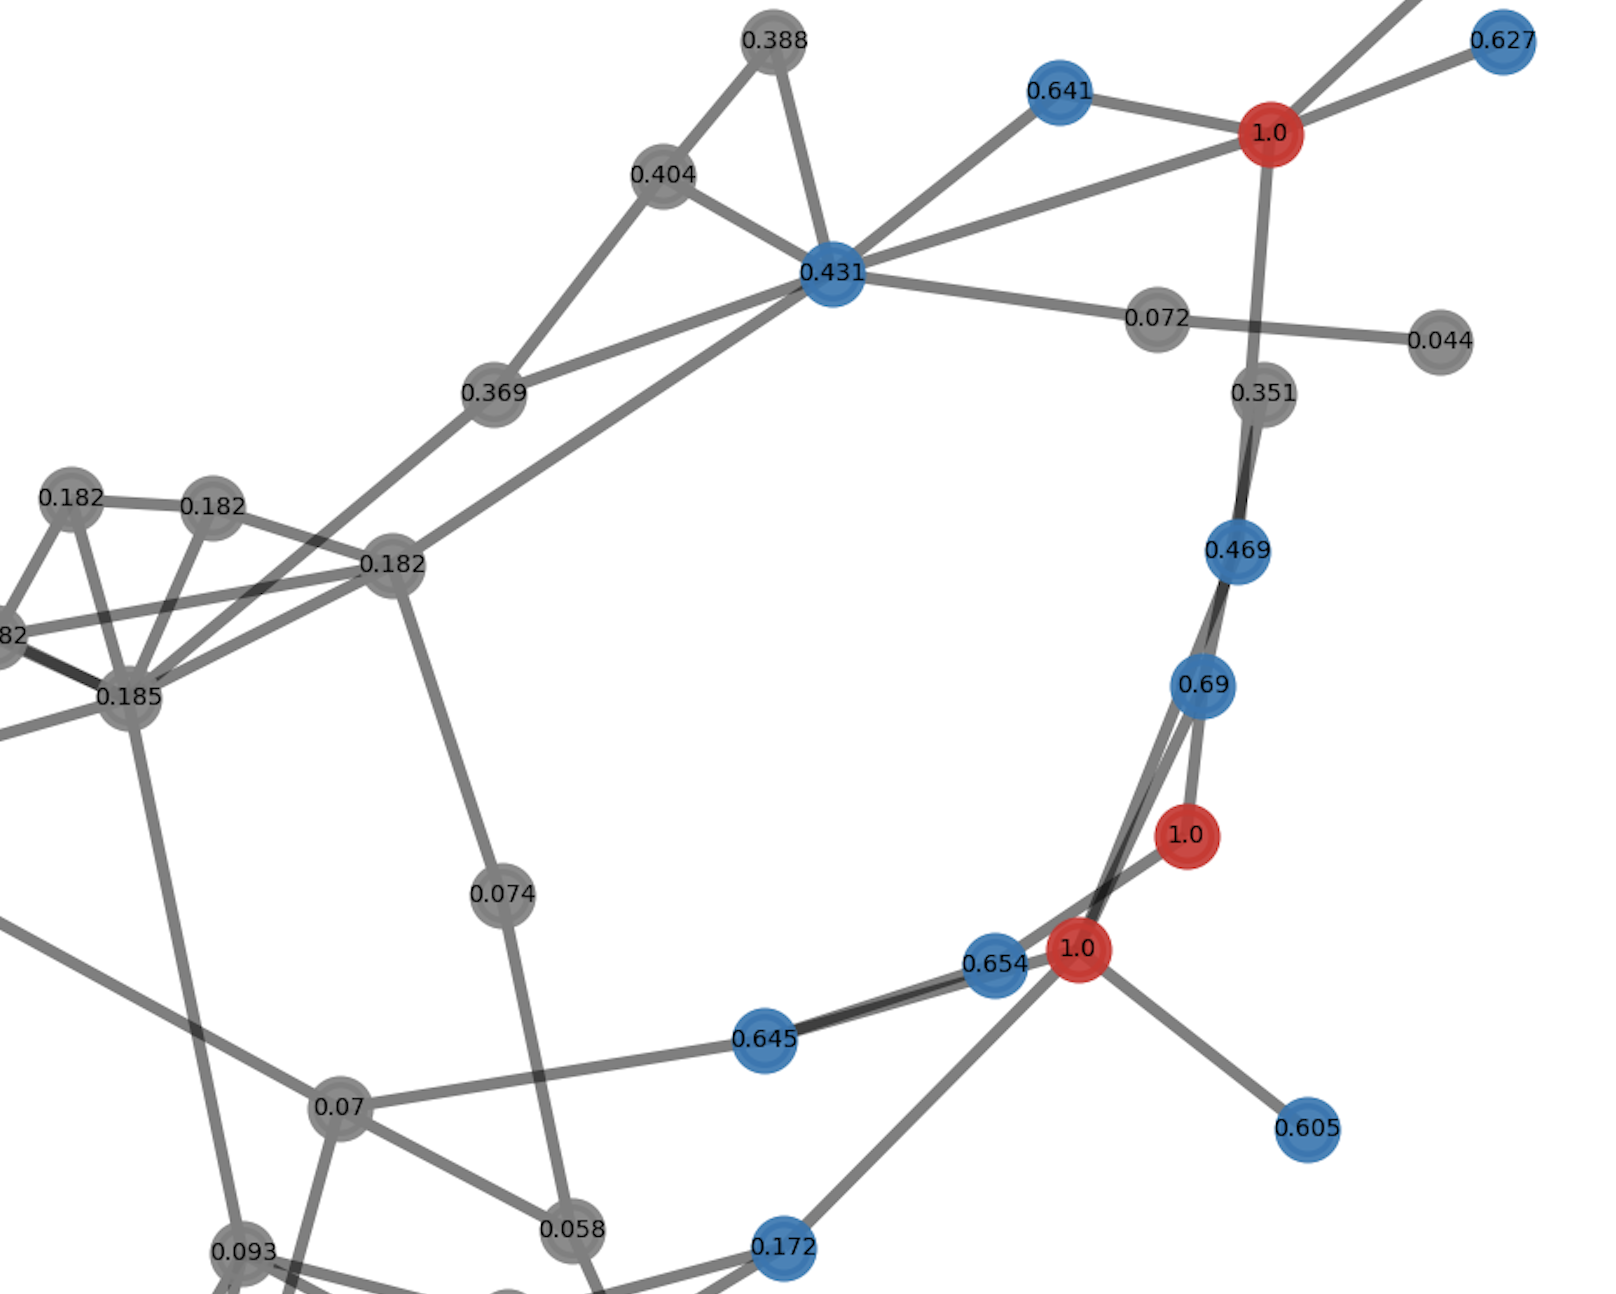
\includegraphics[width=0.7\linewidth]{example.png}
		\caption{Exposure Probabilities}
	\end{figure}
\end{frame}

\begin{frame}
	\frametitle{Estimating Causal Effects}
	\begin{itemize}
		\setlength\itemsep{1em}
		\item With the exposure probabilities, we can estimate ATE ($\rho$) as: \begin{align*}
			y_i = \alpha + \rho Z_i + \gamma (1 - Z_i) \pi_i + \varepsilon_i 
		\end{align*}
		\item $\gamma$ doesnt have any real causal interpretation :(
		\item Much better suited to heterogeneous spillover effects 
		\item Test by simulating data on two real-world social networks \\[0.5ex]
		\begin{itemize}
		\setlength\itemsep{0.5em}
			\item Eighth Graders: 55 students with edges between those who wanted to sit next to each other in class 
			\item Aarhus Computer Science Department: 60 colleagues with edges between those who got lunch together in a given week 
			\item $y_i \sim \mathcal{N}(\mu, \sigma^2)$, $\rho = 3$, spillover = $1.5$
		\end{itemize}
	\end{itemize}
\end{frame}

\begin{frame}
	\frametitle{Simulation Results}
	\resizebox{\textwidth}{!}{
	% \begin{table}
	% 	\caption{Simulation Results (True parameter: $\rho = 3$)}
	% 	\label{table1}
		% \centering
		\begin{tabular}{ccccccc}
		  \toprule
		  & & \multicolumn{2}{c}{Eighth Graders} & & \multicolumn{2}{c}{Aarhus CS}              \\
		  \cmidrule{3-4} \cmidrule{6-7}
		  DGP & $\phi_{i,j}$ & $\bar{y}^1 - \bar{y}^0$ & $\rho$ & & $\bar{y}^1 - \bar{y}^0$ & $\rho$ \\
		  \midrule
		  \multirow{ 2}{*}{Neighbors} & Latent & 2.67 (0.22) & 3.03 (0.30) & & 2.31 (0.21) & 3.03 (0.43)    \\
		  \cmidrule{2-7}
		  & Beta & 2.66 (0.22) & 3.14 (0.38) & & 2.32 (0.21) & 3.63 (0.63)  \\
		  \midrule
		  \multirow{ 2}{*}{Latent}& Latent & 2.73 (0.22) & 2.93 (0.33)  & & 2.55 (0.21) & 2.93 (0.43)  \\
		  \cmidrule{2-7}
		  & Beta  & 2.72 (0.22) & 2.95 (0.35)  & & 2.54 (0.21) & 3.08 (0.61) \\
		  \midrule
		  \multirow{ 2}{*}{$p_{i,j} = 0.5$}& Latent & 2.55 (0.22) & 2.67 (0.38)  & & 2.31 (0.21) & 2.48 (0.46) \\
		  \cmidrule{2-7} 
		  & Beta  & 2.56 (0.23)& 2.81 (0.40)  & & 2.32 (0.21) & 2.64 (0.67)  \\
		  \midrule
		  \multirow{ 2}{*}{No Spillover}& Latent & 3.00 (0.21) & 3.00 (0.24)  & & 3.01 (0.19) & 3.01 (0.27) \\
		  \cmidrule{2-7} 
		  & Beta  & 3.00 (0.20) & 3.00 (0.25)  & & 2.99 (0.19) & 2.99 (0.38)  \\
		  \bottomrule
		\end{tabular}
	% \end{table}
	}
\end{frame}

\begin{frame}
	\frametitle{Simulation Results: Heterogeneous Spillover}
	\resizebox{\textwidth}{!}{
	\begin{tabular}{cccccccc}
		\toprule
		& \multicolumn{3}{c}{Eighth Graders} & & \multicolumn{3}{c}{Aarhus CS}              \\
		\cmidrule{2-4} \cmidrule{6-8}
		$\phi_{i,j}$ & $\bar{y}^1 - \bar{y}^0$ & $\rho$ & $\gamma$ & & $\bar{y}^1 - \bar{y}^0$ & $\rho$ & $\gamma$ \\
		\midrule
		 Latent & 2.74 (0.21) & 2.95 (0.25) & 1.40 (0.39) & & 2.64 (0.20) & 2.99 (0.31) & 0.48 (0.25)    \\
		\cmidrule{1-8}
		Beta & 2.75 (0.21) & 2.99 (0.28) & 0.84 (0.40) & & 2.65 (0.20) & 3.06 (0.38) & 0.51 (0.36) \\
		\bottomrule
	\end{tabular}
	}
\end{frame}

%----------------------------------------------------------------------------------------
%	CLOSING SLIDE
%----------------------------------------------------------------------------------------

\begin{frame}[plain] % The optional argument 'plain' hides the headline and footline
	\begin{center}
		{\Huge The End}
		
		% \bigskip\bigskip % Vertical whitespace
		
		% {\LARGE Questions? Comments?}
	\end{center}
\end{frame}

%----------------------------------------------------------------------------------------

\end{document}